 % !TEX encoding = UTF-8 Unicode
% !TeX spellcheck = pl_PL
% !~~TEX TS-program = xelatex
% !TeX TXS-program:bibliography = txs:///biber
% !TeX TXS-program:index = txs:///makeindex

\documentclass[skorowidz,skroty]{dyplomWEZUT}
% ------------------------------------------------------------------------------
% Opcje klasy <dyplomWEZUT>
% 1) skorowidz - włącza skorowidz
% 2) skroty    - włącza wykaz ważniejszych skrótów i oznaczeń
% ------------------------------------------------------------------------------


% -------------------------- Dane pracy dyplomowej -----------------------------

% Imię i Nazwisko
\author{Adam Baniuszewicz}

% Numer albumu
\nralbumu{33816}

% Tytuł pracy
\title{Algorytmy poleceń mentalnych w~interfejsach mózg--komputer}

% Tytuł pracy w języku angielskim
\tytulang{Algorithms of~mental commands in~brain--computer interfaces}

% Kierunek studiów
\kierunek{Teleinformatyka}

% Rodzaj studiów: S1/S2/N1/N2
\rodzajstudiow{S2}

% Specjalność (tylko na studiach magisterskich - S2 i N2)
\specjalnosc{Sieci teleinformatyczne i~systemy mobilne}

% Data wydania tematu w SIWE/eDziekanacie
\datawydania{01.11.2018}

% Data złożenia pracy w eDziekanacie
\datazlozenia{TODO}

% Miejsce złożenia pracy (odkomentować i wypełnić jeżeli inne niż Szczecin)
%\miejsce{}

% Imię i nazwisko opiekuna - wpisujemy w dopełniaczu
\opiekun{dr. inż. Roberta Krupińskiego}

% Katedra, Zakład lub Zespół Dydaktyczny
% (Wydział wpisujemy po przecinku tylko jeśli inny niż WE)
\jednostka{Katedra Przetwarzania Sygnałów i~Inżynierii Multimedialnej}

% Słowa kluczowe
\slowakluczowe{BCI, Elektroencefalografia}

% Słowa kluczowe po angielsku
\keywords{BCI, Electroencephalography}

%% ----------------------- Koniec definicji danych -----------------------------

% Dodanie metadanych do wynikowego pdf (Autor, Tytuł, Słowa kluczowe)
\makemetadata

\begin{document}

\begin{streszczenie}
TODO
\end{streszczenie}

\begin{abstract}
TODO
\end{abstract}

\maketitle

\begin{wprowadzenie}

TODO

\end{wprowadzenie}

\cel{TODO}

\zakres{TODO}

\chapter{Wstęp do tematyki interfejsów mózg--komputer}
\section{Czym jest BCI}
\section{Podział BCI ze względu na sposób akwizycji sygnałów}
\subsection{Nieinwazyjne}
\subsection{Inwazyjne}
\subsection{Stymulujące oraz dwukierunkowe}

\section{Przetwarzanie sygnałów}
\subsection{Usunięcie szumów}
Sygnały EEG charakteryzują się bardzo niskim współczynnikiem SNR\footnote{SNR (\textit{ang.} signal-to-noise ratio) -- stosunek sygnału do szumu}\cite{bci_trends}. Z tego powodu przed przystąpieniem do ich analizy należy najpierw usunąć z nich możliwie największą ilość artefaktów. Przykładowe przebiegi zakłóceń zostały pokazane na rysunku \vref{fig:eeg_noise}.

Pierwszym typem zakłóceń są zakłócenia pochodzące ze środowiska, w którym jest rejestrowany sygnał EEG. Możemy do nich zaliczyć między innymi zakłócenia od sieci energetycznej oraz elektroniki (komputerów, telefonów, routerów Wi-Fi i tym podobnych). Najprostszym sposobem minimalizacji ich wpływu na sygnał wyjściowy jest eliminacja źródeł zakłóceń -- przeprowadzenie akwizycji sygnałów z dala od miast, usunięcie zbędnych urządzeń z otoczenia, zastąpienie, o ile to możliwe, zasilania niezbędnych urządzeń prądem przemiennym na rzecz prądu stałego. Innym sposobem jest wykorzystanie klatki Faradaya.

Drugim typem zakłóceń są tak zwane zakłócenia fizjologiczne. Powstają one na skutek ruchu ciała lub innych fluktuacji potencjałów bioelektrycznych. Ich źródła są niemożliwe do wyeliminowania. Typowymi przykładami takich zakłóceń są sygnały EOG, EMG oraz EKG. W szczególności dwa pierwsze, z racji małej odległości od miejsca akwizycji sygnałów EEG, mają duży wpływ na SNR. Wpływ EOG oraz EMG można zminimalizować poprzez uniknięcie nadmiernego mrugania, ruchu oczu oraz napinania mięśni.

Typowymi technikami usunięcia artefaktów z sygnału EEG są\cite{bci_introduction}:
\begin{description}
    \item [Progowanie] --- jeżeli jakakolwiek charakterystyka sygnału EOG lub EMG przekracza zdefiniowany próg (\textit{ang.} threshold), próbki sygnałów EEG w tej epoce zostają uznane za skażone i są odrzucane. Ten sposób może być zastosowany również dla akwizycji wyłącznie sygnałów EEG, jednak to podejście wymaga wstępnej kalibracji z użytkownikiem. Wadą tego rozwiązania jest utrata informacji zawartych w odrzuconych próbkach.
    
    \item [Filtracja] --- wycięcie z pobranego sygnału składowych o określonym paśmie częstotliwości przy użyciu filtru pasmowo--zaporowego. W celu przeprowadzenia filtracji należy przekształcić sygnał do dziedziny częstotliwości (na przykład przy użyciu FFT), wyciąć składowe o niepożądanej częstotliwości, a następnie przekształcić sygnał z powrotem do dziedziny czasu. Usunąć w ten sposób można między innymi zakłócenia sieci energetycznej\footnote{W zależności od kraju zakłócenia te mogą występować w innym paśmie częstotliwości. W Europie jest to 50 Hz, ale na przykład w większości państw Ameryki Północnej częstotliwość sieci wynosi 60 Hz.} oraz artefakty EOG (około 1÷4 Hz). Filtrację należy stosować, tylko jeżeli podlegające jej składowe mają inną częstotliwość niż sygnały, które chcemy uzyskać.
    
    \item [Regresja liniowa] --- przy założeniu, iż szum sygnału EEG jest addytywny można sformułować zależność w postaci\cite{bci_introduction}:
    $$ EEG_i(t) = EEG^{true}_i(t) + K \times EOG(t) $$
    gdzie $EEG^{true}_i(t)$ jest \textit{czystym} sygnałem EEG pozyskanym z elektrody $i$ w czasie $t$, $EOG(t)$ jest sygnałem EOG w czasie $t$, a $K$ stałą, która może być estymowana. Posiadając estymację stałej $K$, na podstawie prostego przekształcenia możemy uzyskać estymację czystego sygnału EEG w postaci:
    $$ EEG^{true}_i(t) = EEG_i(t) - K \times EOG(t) $$
    Ten sposób trudniejszy do usunięcia artefaktów EMG, ponieważ pochodzą one z wielu źródeł (wielu grup mięśni) i wymagają opracowania bardziej skomplikowanego modelu.

    \item [Analiza składowych głównych] --- inaczej PCA (\textit{ang.} Principal Component Analysis); polega na redukcji współczynników potrzebnych do opisania dużej liczby skorelowanych ze sobą zmiennych, przy jednoczesnym zachowaniu jak największej liczby składowych znajdujących się w sygnale właściwym. Umożliwia zmniejszenie ilości informacji zawartych w sygnale poprzez eliminację pewnych składowych zawierających artefakty\cite{eeg_noise}. PCA pozwala na usunięcie szumów związanych z EOG\cite{bci_introduction}.
    
    \item [Analiza składowych niezależnych] --- inaczej ICA (\textit{ang.} Independent Component Analysis); pozwala na estymację nieznanych sygnałów źródłowych oraz ekstrakcje zakłóceń w celu ich późniejszej eliminacji\cite{eeg_noise}. ICA stosuje się w celu eliminacji zakłóceń EOG oraz EMG\cite{bci_introduction}.
\end{description}

% rysunek z szumami EEG
\begin{figure}[htb]
    \begin{subfigure}{0.48\textwidth}
    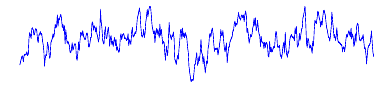
\includegraphics[width=\linewidth]{graphic/eeg_noise_clean}
    \caption{Czysty sygnał EEG}
    \end{subfigure}\hspace*{\fill}
    \begin{subfigure}{0.48\textwidth}
    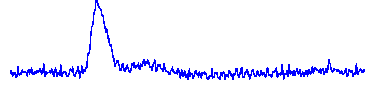
\includegraphics[width=\linewidth]{graphic/eeg_noise_blink}
    \caption{Mrugnięcie}
    \end{subfigure}
    
    \medskip
    \begin{subfigure}{0.48\textwidth}
    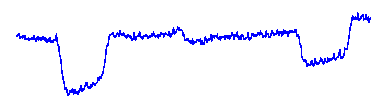
\includegraphics[width=\linewidth]{graphic/eeg_noise_eye}
    \caption{Ruch gałki ocznej}
    \end{subfigure}\hspace*{\fill}
    \begin{subfigure}{0.48\textwidth}
    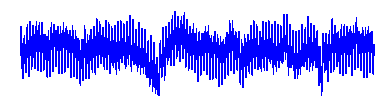
\includegraphics[width=\linewidth]{graphic/eeg_noise_line}
    \caption{Zakłócenia sieci energetycznej}
    \end{subfigure}
    
    \medskip
    \begin{subfigure}{0.48\textwidth}
    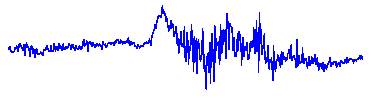
\includegraphics[width=\linewidth]{graphic/eeg_noise_muscle}
    \caption{Aktywność mięśni}
    \end{subfigure}\hspace*{\fill}
    \begin{subfigure}{0.48\textwidth}
    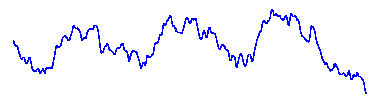
\includegraphics[width=\linewidth]{graphic/eeg_noise_pulse}
    \caption{Tętno}
    \end{subfigure}
    
    \caption{Rodzaje artefaktów występujących w sygnałach EEG\label{fig:eeg_noise}}
    \source{\cite{eeg_artifact}}
\end{figure}


\subsection{Ekstrakcja cech}
Celem ekstrakcji cech jest przekształcenie \textit{surowych} danych EEG do postaci nadającej się do wykorzystania w procesie klasyfikacji sygnałów\cite{bci_robotics}. Cecha jest właściwością opisującą sygnał EEG\cite{bci_foundations}, na przykład jego amplitudą lub rozkładem widmowym. Cechy są zazwyczaj grupowane w wektory cech\cite{bci_foundations}. Przykładem wykorzystania ekstrakcji cech może być rozpoznanie wyobrażenia ruchu ręką -- cechą używaną do detekcji jest moc pasma μ (8÷12 Hz) oraz β (16÷24 Hz)\cite{bci_foundations}.

W interfejsach mózg--komputer najczęściej wykorzystywane są cechy opisujące sygnał\cite{eeg_features}:
\begin{description}
    \item [Przestrzennie] --- służą do przybliżonego wyznaczania źródeł sygnału\cite{eeg_features}.
    \item [Spektralnie] --- opisują moc sygnału w zależności od częstotliwości\cite{bci_foundations}.
    \item [Czasowo] --- opisują zmianę sygnału w czasie.
\end{description}

Innymi cechami wykorzystywanymi w BCI są reprezentacje czasowo--czę\-sto\-tli\-wo\-ścio\-we sygnałów, transformacja Hilberta oraz parametry Hjortha\cite{bci_robotics}. 


\subsection{Klasyfikacja sygnałów}

\section{Przegląd potencjalnych zastosowań}
\subsection{Interfejs komunikacyjny}
Najprostsze interfejsy komunikacyjne można zrealizować dając użytkownikowi do wyboru dwie opcje: \textit{tak} lub \textit{nie}. Podejście dwuwartościowe pozwala na stosowanie różnorodnych technik akwizycji wyboru, między innymi poprzez analizę mrugnięć, ruchu gałek ocznych, czy sygnałów pochodzących z BCI. Przy tak skonstruowanym interfejsie osoba z niego korzystająca jest w stanie odpowiadać na pytania rozmówcy.

Taki sposób komunikacji może być zmodyfikowany w celu umożliwienia osobie użytkującej interfejs nadawania toku rozmowy. Dzięki zastosowaniu tablicy ze znakami, jej rozmówca może przemieszczać  po kolei swój palec po literach alfabetu i notować te, dla których osoba korzystająca z interfejsu zakomunikowała odpowiedź \textit{tak}. Wadą takiego rozwiązania jest fakt, iż rozmówca musi asystować osobie niepełnosprawnej, co może wprowadzać uczestników rozmowy w zakłopotanie. Taki interfejs charakteryzuje się małą stopą błędu, jednak komunikacja przy jego użyciu jest długotrwała i wynosi około jedno słowo na minutę\cite{bci_trends}.

Innym podejściem jest stworzenie systemu opartego o wirtualny kursor, który pozwoliłby użytkownikowi na samodzielnie wybieranie liter lub całych wyrazów spośród dostępnych opcji. Taki system może zawierać elementy autokorekty, aby zminimalizować występujące błędy.

W literaturze można również spotkać się z systemami badającymi potencjały wymuszone. Taką metodą jest \textit{P300}. W takim interfejsie użytkownik skupia swoją uwagę na literze, którą chce wybrać. Litery są samoczynnie podświetlane w losowej kolejności. 300 milisekund po podświetleniu litery, na której użytkownik systemu jest aktualnie skupiony, można zaobserwować zmianę amplitudy rejestrowanego sygnału EEG\cite{bci_introduction}. Przykładową realizację interfejsu opartego o analizę potencjału P300 pokazano na rysunku \vref{fig:p300_interface}.

\rysunek{p300}
{Struktura interfejsu opartego o potencjał P300\label{fig:p300_interface}}
{\cite{p300_interface}}


\subsection{Sterowanie wózkiem inwalidzkim}
Osoby sparaliżowane niekiedy są w stanie sterować wózkiem inwalidzkim, używając do tego celu wydmuchiwanego powietrza, mowy lub, w przypadku częściowego paraliżu, sprawnych części ciała. Integracja z interfejsami mózg--komputer stwarza nowe możliwości dla osób, które z powodu poważniejszych schorzeń nie są w stanie skorzystać z wyżej wymieniowych metod sterowania.

Kontrola wózka inwalidzkiego może odbywać się przy wykorzystaniu sterowania \textit{nisko-} lub \textit{wysokopoziomowego}.

Sterowanie niskopoziomowe można zrealizować przez translację sygnałów odebranych z urządzenia rejestrującego aktywność mózgu na komendy opisujące ruch wózka (\textit{ruch do przodu}, \textit{zawróć}, \textit{przyspiesz}), z zastrzeżeniem, że użytkownik wydaje je w sposób bezpośredni. Ten rodzaj sterowania wymaga zamontowania czujników na wózku, które uniemożliwią wykonanie niedozwolonych manewrów, na przykład uderzenia w inną osobę lub przedmiot. Do zalet rozwiązania można zaliczyć wysoki stopień kontroli osoby użytkującej wózek nad sposobem przemieszczania oraz stosunkowo małą ilość wymaganych komend mentalnych do podstawowego sterowania. Do wad należy konieczność wydawania poleceń ruchu w sposób ciągły, co może prowadzić do znużenia użytkownika, a w konsekwencji samoczynnego \textit{rozstrajania się} układu sterowania.

Sterowanie wysokopoziomowe polega na wydawaniu poleceń dotyczących celu ruchu (\textit{kuchnia}, \textit{łazienka}). Podejście to wiąże się z koniecznością stosowania wózków o wysokim stopniu autonomiczności. Zaletą tego rozwiązania jest odciążenie użytkownika od konieczności utrzymywania ciągłego skupienia na kierunku oraz prędkości ruchu, wyeliminowanie wpływu zakłóceń odbieranych w trakcie przemieszczania się oraz, po zapewnieniu skutecznych algorytmów i odpowiedniej ilości czujników, bezpieczniejsze poruszanie się w środowisku. Do wad zaliczyć należy większą ilość komend, które należy zdefiniować (co najmniej po jednej dla każdego pomieszczenia), mniejszą precyzję ruchu, spowodowaną odgórnym określeniem miejsca w pomieszczeniu, do którego użytkownik chce się przemieścić oraz konieczność zdefiniowania i zmapowania każdego środowiska, w którym będzie poruszał się wózek.

Mimo obiecujących wstępnych rezultatów, wykorzystanie interfejsów mózg--kom\-pu\-ter do zadania sterowania wózkami inwalidzkimi jest trudne do zrealizowania z powodu braku niezawodnych, przenośnych i łatwych w użyciu urządzeń rejestrujących. Inną przeszkodą jest brak wózków o wystarczającym stopniu autonomiczności, które byłyby zdalne do pracy w codziennym środowisku\cite{bci_introduction}.


\subsection{Rehabilitacja}
Można wyróżnić trzy główne sposoby wsparcia rehabilitacji medycznej przez interfejsy mózg--komputer\cite{bci_lab}:
\begin{description}
    \item [mózg--akcja] --- polega na nauczeniu pacjenta przy pomocy BCI wydawania odpowiednich poleceń, wymaganych do usprawnienia motoryki kończyn,
    \item [mózg--kończyna] --- polega na wykorzystaniu BCI do kontroli urządzenia wspierającego poruszanie się, a w konsekwencji odbudowania połączeń potrzebnych do poruszania się bez niego,
    \item [mózg--mózg] --- na podstawie informacji odebranych z systemu BCI następuje stymulacja mózgu w celu poprawy jego aktywności, aż do osiągnięcia zadowalających rezultatów.
\end{description}
Należy nadmienić, iż te sposoby nie wykluczają się wzajemnie -- ich połączenie pozwala na zwiększenie znaczenia BCI w tej dziedzinie nauki.

Interfejsy mózg--komputer, poprzez stopniową integrację z neurorehabilitacją, mogą pomóc między innymi osobom dotkniętym udarem mózgu, który często powoduje długotrwałą niepełnosprawność ruchową oraz zaburzenia funkcji poznawczych. Wiele badań wykazuje, iż technika nieinwazyjnej stymulacji mózgu jest skuteczna, nawet w przypadku przewlekłego uszkodzenia mózgu\cite{bci_lab}. Duża ilość osób rokrocznie dotykanych udarem stanowi badania w tym zakresie niezwykle istotnymi dla społeczeństwa.

Stosowanie BCI do wspomagania leczenia funkcji poznawczych wymaga skrupulatnej identyfikacji sygnałów mózgowych, które są możliwe do uzyskania. Może to być trudne, ponieważ nie wszystkie stany mózgu są tak dobrze scharakteryzowane, jak te związane z funkcjami motorycznymi\cite{bci_handbook}.


\subsection{Nadzór skupienia}
Wykorzystanie interfejsów mózg--komputer do nadzorowania skupienia użytkownika jest szczególnie istotne w asystowaniu pracowników wykonujących monotonne prace, takie jak prowadzenie samochodu czy monitorowanie systemu zabezpieczeń. Popełnienie błędu w przypadku takich profesji powoduje nie tylko ryzyko dla samego pracownika, ale również dla innych osób znajdujących się w jego otoczeniu. Wiele wypadków jest spowodowanych zmęczeniem, nieuwagą lub nawet zaśnięciem podczas wykonywania pracy. Choć znużenie lub senność może być wykryta przez analizowanie obszaru okolic oczu, taka detekcja może mieć miejsce za późno, aby było możliwe zapobiegnięcie wypadkowi. Integracja BCI z urządzeniami do nadzoru niesie możliwość wykrywania takich sytuacji, zanim doprowadzą do katastrofalnych w skutkach wydarzeń. 

W związku z postępującą automatyzacją pojazdów, kierowca jest odciążany od wykonywania żmudnych zadań, takich jak utrzymywanie stałej prędkości czy przełączanie między światłami mijania oraz drogowymi. Wraz z dalszym progresem coraz więcej czynności wykonywanych jest przez sam samochód, podczas kiedy rola osoby znajdującej się w fotelu kierowcy sprowadza się do nadzoru i reagowania w niebezpiecznych sytuacjach. Może to prowadzić, w szczególności na trasach o znacznej długości, do sytuacji nadmiernego zaufania do systemu sterowania, w której to kierowca przestanie zwracać uwagę na działania pojazdu. Interfejs mózg--komputer mógłby w tym momencie sygnalizować spadek skupienia kierowcy lub wymuszać bezpieczny postój pojazdu do momentu, w którym kierujący pojazdem będzie w stanie kontynuować podróż.

Badania przeprowadzone przez naukowców z \textit{Berlin BCI} wykazały, iż istnieje zależność pomiędzy spadkiem koncentracji, a wzrostem mocy w paśmie alpha\footnote{Pasmo alpha - pasmo fal elektromagnetycznych o częstotliwości 8÷12 Hz i amplitudzie w zakresie 20÷80 μV\cite[str. 17]{bci_handbook}.}\cite{berlinbci_attention}. Badanie polegało na sklasyfikowaniu 2000 bagaży jako bezpiecznych lub niebezpiecznych na podstawie ich prześwietleń. Wykonano je w 10 turach po 200 bagaży. Na podstawie rysunku \vref{fig:attention} można wywnioskować, iż spadek koncentracji (wzrost parametru CII) prowadził do wzmożenia ilości popełnianych błędów. Uczestnicy rzeczonego badania na okres następujący bezpośrednio po przerwie wykazywali znacznie niższy stopień błędu. Tę zależność można wykorzystać do określenia momentów, w których pracownik powinien udać się na przerwę lub, w przypadku długotrwałej nikłej koncentracji, zakończyć swoją zmianę.

\rysunekbig{attention}
{Zależność pomiędzy stopniem skupienia CII (\textit{ang.} concentration insufficiency index), a stopą błędu. Pionowe linie po zakończeniu dwustupróbkowych bloków oznaczają moment przerwy.\label{fig:attention}}
{\cite{berlinbci_attention}}


\subsection{Gry komputerowe}
Wprowadzenie dedykowanych rozwiązań dla przemysłu gier komputerowych wydaje się być kolejnym krokiem po rozwoju aplikacji korzystających z technologii VR\footnote{VR (\textit{ang.} virtual reality) -- rzeczywistość wirtualna} oraz AR\footnote{AR (\textit{ang.} augmented reality) -- rzeczywistość rozszerzona}. To, co sprawia, że gracze są odpowiednim odbiorcą wczesnych systemów BCI jest fakt, iż często są oni zainteresowani nowymi technologiami, są skłonni do jej wdrażania w celu uzyskania przewagi nad przeciwnikami oraz przyzwyczajeni do konieczności treningu, który pozwala na progres w grach\cite{bci_games_survey}. W związku z dynamicznym rozwojem tej branży, opracowanie rozwiązań wykorzystujących BCI może być bardzo opłacalne w przyszłości.

Wykorzystanie BCI w grach komputerowych pozwala na integrację gry z wrażeniami użytkownika. Dostarczenie informacji na temat skupienia, zainteresowania, frustracji czy znudzenia umożliwia grze dostosowanie się do potrzeb gracza. W przypadku narastania frustracji gra może samoczynnie obniżyć poziom trudności, a w przypadku znudzenia -- podwyższyć. Wykorzystując inne odczucia gra może również uprościć interfejs użytkownika, czy też wyświetlić lub ukryć podpowiedzi dotyczące aktualnie wykonywanego zadania (\textit{ang.} quest). Dynamiczne dostosowywanie gry do aktualnego stanu gracza pozwala jej na zapewnienie użytkownikowi zwiększonego komfortu podczas rozgrywki.

Innym zastosowaniem interfejsów mózg--komputer jest wydawanie poleceń za pomocą komend mentalnych. Poleceniem może być na przykład wyobrażenie sobie ruchu postaci, co prowadziłoby do faktycznego przemieszczania się kontrolowanego bohatera, czy wybieranie odpowiedzi w dialogach występujących w grze. Wiąże się to z całkowitą zależnością gry od sygnałów otrzymywanych z urządzenia rejestrującego i wnosi konieczność znacznej modyfikacji istniejących silników gier.

Zintegrowanie BCI z grami komputerowymi wiąże się nie tylko ze znacznymi inwestycjami ze strony producentów gier, ale również samych graczy, którzy będą musieli zakupić urządzenia rejestrujące aktywność mózgu. Należy zwrócić uwagę na fakt, że rozgrywki często prowadzone są przez długi okres, a więc wymogiem stawianym przed systemami rejestrującymi jest ich wygoda. Nie mogą one ograniczać ruchów użytkownika ani jego pola widzenia. Wadą rozwiązania jest fakt, iż gracze często generują napięcia mięśniowe, co będzie prowadziło do powstawania artefaktów w przypadku urządzeń rejestrujących sygnały EEG. Rozwiązaniem tego problemu może być ulepszenie algorytmów filtracji sygnałów lub stosowanie systemów hybrydowych EEG/EMG, a więc rejestrujących oraz wykorzystujących aktywność zarówno mózgu, jak i mięśni\cite{bci_introduction}.


\chapter{Charakterystyka wybranych urządzeń komercyjnych}
\section{Emotiv Insight\label{section:insight}}
Insight (patrz rysunek \vref{fig:insight}) jest produktem wprowadzonym na rynek w roku 2015 przez firmę Emotiv przy wsparciu crowdfundingu na portalu \href{www.kickstarter.com}{kickstarter}. Jest produktem do użytku codziennego, głównie za sprawą minimalistycznego designu oraz braku konieczności stosowania żelów przewodzących, przeznaczonym do mniej precyzyjnych zastosowań.

Jest wyposażony w pięć czujników właściwych oraz dwa referencyjne. Lokalizacja czujników została przedstawiona na rysunku \vref{fig:insight_area}. Czas ubrania oraz ustawienia urządzenia oscyluje w granicach 1--2 minut. Parametry urządzenia zostały zestawione w tabeli \vref{tab:insight}.

Koszt produktu na dzień 21 kwietnia 2019 roku wynosi 299\$.

\rysunekbig{insight}
{Hełm Emotiv Insight\label{fig:insight}}
{\cite{emotiv_insight}}

\rysunekbig{insight_area}
{Rozmieszczenie sensorów w hełmie Emotiv Insight\label{fig:insight_area}}
{\cite{emotiv_insight}}

\tabela{Parametry Emotiv Insight\label{tab:insight}}
{Opracowanie własne na podstawie \cite{emotiv_comparison}}
{
    \begin{tabular}{l|l}
        Ilość kanałów & 5 (+2 referencyjne)\\
        Umiejscowienie elektrod & AF3, AF4, T7, T8, Pz\\
        Czujniki referencyjne & DMS/DRL\\
        Rodzaj czujników & Półsuchy polimer\\
        Rozdzielczość & 14 bit na kanał\\
        Rozdzielczość LSB & 0,51 µV @ 14 bit\\
        Detekcja ruchu & 9-osiowy czujnik (3x żyroskop, 3x akcelerometr, 3x magnetometr)\\
        Łączność & Bezprzewodowa 2,4GHz/Bluetooth 4.0\\
        Zasilanie & Li-Pol 480 mAh, do 8 godzin pracy
    \end{tabular}
}

Firma Emotiv dostarcza do swoich rozwiązań API\footnote{API (\textit{ang.} application programming interface) -- Interfejs programistyczny aplikacji. Zawiera zestaw reguł i ich opisów, które definiują sposób komunikacji między programami komputerowymi.\label{foot:api}} o nazwie Cortex. Stanowi on podstawę do budowania aplikacji wykorzystujących pobrane z hełmów strumienie danych dzięki wykorzystaniu JSON oraz WebSocket\cite{emotiv_developer}. Cortex ułatwia tworzenie gier, aplikacji oraz rejestrowania danych do późniejszego ich wykorzystania do badań.

Cortex jest wrapperem SDK\footnote{SDK (\textit{ang.} software development kit) -- Zestaw narzędzi dla programistów niezbędny w tworzeniu aplikacji korzystających z danej biblioteki.\label{foot:sdk}} firmy EMOTIV. Zapewnia on, w zależności od rodzaju zakupionej licencji, dostęp do różnych strumieni danych z hełmów. Jest kompatybilny z systemami Mac OS oraz Windows. Umożliwia programowanie w językach Java, C\#, C++, Python, Ruby, JavaScript (Node.js) oraz PHP.

Licencja Cortex jest dostępna w trzech planach:
\begin{description}
    \item [Darmowa] \hfill
    \begin{itemize}
        \item Mental Commands API,
        \item Performance Metrics API (do 0,1 Hz),
        \item Frequency Bands API,
        \item Facial Expressions API,
        \item Motion data API,
        \item nielimitowana ilość sesji na 3 urządzeniach.
    \end{itemize}
    \item [Niekomercyjna pro -- \$55-99/miesiąc] \hfill
    \begin{itemize}
        \item Wszystkie API z licencji darmowej,
        \item Raw EEG API,
        \item oprogramowanie EmotivPRO,
        \item nielimitowana ilość sesji na 3 urządzeniach.
    \end{itemize}
    \item [Komercyjna] \hfill
    \begin{itemize}
        \item Performance Metrics API o wysokiej rozdzielczości,
        \item konfigurowanie API pod swoje potrzeby,
        \item tworzenie komercyjnych rozwiązań.
    \end{itemize}
\end{description}

Oprogramowanie EmotivPRO\cite{emotiv_pro}, dostępne w licencjach niekomercyjnej pro oraz komercyjnej, stanowi wsparcie dla badań wykorzystujących EEG. Pozwala ono na akwizycję oraz prezentację strumieni danych w czasie zbliżonym do rzeczywistego, zapisywanie sesji w chmurze oraz szybką analizę wbudowanym algorytmem FFT\footnote{FFT (\textit{ang.} Fast Fourier Transform) -- Szybka transformacja Fouriera.}, bez konieczności eksportu danych.


\section{Emotiv EPOC+\label{section:epoc}}
EPOC+, pokazany na rysunku \vref{fig:epoc}, został wprowadzony na rynek w 2013 roku przez firmę Emotiv. Został zaprojektowany do badań wykorzystujących EEG oraz zaawansowanych zastosowań BCI\cite{emotiv_epoc}.

Jest wyposażony w 14 kanałów właściwych oraz 2 referencyjne (dokładna lokalizacja sensorów została przedstawiona na rysunku \vref{fig:epoc_area}). W odróżnieniu od Emotiv Insight, omówionego w rozdziale \vref{section:insight}, wymaga stosowania \textit{mokrych} elektrod, pokrytych nasączonym solą fizjologiczną filcem. Ze względu na większą ilość czujników niż w Emotiv Insight, czas ubrania oraz przygotowania urządzenia do pracy wynosi około 3--5 minut. Parametry hełmu zostały przedstawione w tabeli \vref{tab:epoc}.

Koszt produktu na dzień 21 kwietnia 2019 roku wynosi 799\$.

\rysunekbig{epoc}
{Hełm Emotiv EPOC+\label{fig:epoc}}
{\cite{emotiv_epoc}}

\rysunekbig{epoc_area}
{Rozmieszczenie sensorów w hełmie Emotiv EPOC+\label{fig:epoc_area}}
{\cite{emotiv_epoc}}

\tabela{Parametry Emotiv EPOC+\label{tab:epoc}}
{Opracowanie własne na podstawie \cite{emotiv_comparison}}
{
    \begin{tabular}{l|l}
        Ilość kanałów & 14 (+2 referencyjne)\\
        Umiejscowienie elektrod & AF3, AF4, F3, F4, FC5, FC6, F7, F8, T7, T8, P7, P8, O1, O2\\
        Czujniki referencyjne & DMS/DRL\\
        Rodzaj czujników & Nasączane solą fizjologiczną\\
        Rozdzielczość & 14/16 bit na kanał\\
        Rozdzielczość LSB & 0,51 µV @ 14 bit/0,13 µV @ 16 bit\\
        Detekcja ruchu & 9-osiowy czujnik (3x żyroskop, 3x akcelerometr, 3x magnetometr)\\
        Łączność & Bezprzewodowa 2,4GHz/Bluetooth 4.0\\
        Zasilanie & Li-Pol 680 mAh, do 12 godzin pracy
    \end{tabular}
}

Od strony programistycznej urządzenie wykorzystuje to samo API oraz SDK co Emotiv Insight; zostały one omówione w rozdziale \vref{section:insight}.


\section{Muse/Muse 2}
Muse/Muse 2 są urządzeniami wspomagającymi medytację, które pozwalają na rejestrację w czasie rzeczywistym aktywności mózgu, tętna, oddechu oraz ruchu ciała\footnote{Rejestracja poszczególnych parametrów w zależności od wersji opaski.}\cite{muse2}. Przekształcają one zmierzoną aktywność mózgu w predefiniowane dźwięki, takie jak szum wody czy deszczu; w zależności od poziomu skupienia dźwięk będzie spokojny lub gwałtowny, co pozwala osobom uczącym się medytować na efektywniejszą naukę wyciszenia umysłu.

Oba urządzenia są z wyglądu bardzo do siebie podobne. Nowsze, Muse 2 (pokazane na rysunku \vref{fig:muse2}), w odniesieniu do poprzedniej wersji, zostało \textit{odchudzone}, przez co nabrało bardziej eleganckiego wyglądu oraz zyskało niższy profil z dodatkowymi czujnikami\cite{muse_comparison_article}. Dodano również miękkie w dotyku wykończenie.

\rysunek{muse2}
{Opaska Muse 2\label{fig:muse2}}
{\cite{muse2}}
  
Obie opaski są wyposażone w 7 czujników, w tym 3 referencyjne (patrz rysunek \vref{fig:muse_area}). Zestawienie parametrów oferowanych przez obie opaski znajduje się w tabeli \vref{tab:muse}.

\rysunekbig{muse_area}
{Rozmieszczenie sensorów w opasce Muse\label{fig:muse_area}}
{\cite{muse_specification}}

Koszt Muse wynosi 219€; Muse 2 -- 269€.

\tabela{Parametry Muse oraz Muse 2\label{tab:muse}}
{Opracowanie własne na podstawie \cite{muse_comparison} oraz \cite{muse_specification}}
{
    \begin{threeparttable}
        \begin{tabular}{l|l|l}
            Parametr & Muse & Muse 2 \\\hline\hline
            Ilość kanałów & 4 (+ 3 referencyjne) & 4 (+3 referencyjne)\\
            Umiejscowienie elektrod & TP9, AF7, AF8, TP10\tnote{a} & TP9, AF7, AF8, TP10\tnote{a} \\
            Czujniki referencyjne & CMS/DRL & CMS/DRL \\
            Rodzaj czujników & Suche srebrne/silikonowe & Suche srebrne/silikonowe \\
            Rozdzielczość & 12 bit na próbkę & 12 bit na próbkę \\
            Rejestrowane parametry & EEG & EEG, tętno, ruch ciała, oddech \\
            Kompatybilność & iOS, Android & iOS, Android \\
            Łączność & Bezprzewodowa Bluetooth 4.0 & Bezprzewodowa Bluetooth 5.0 \\
            Zasilanie & Li-Ion, do 5 godzin pracy & Li-Ion, do 5 godzin pracy \\
        \end{tabular}
        \begin{tablenotes}
            \item[a] \footnotesize Dokładna lokalizacja zależy od wielkości głowy użytkownika; zamieszczono lokalizację zgodną z \cite{muse_specification}. W literaturze można spotkać również T9, FP1, FP2, T10\cite{muse_article}.
        \end{tablenotes}
    \end{threeparttable}
}

Muse posiada oferty skierowane do następujących grup:
\begin{description}
    \item [\sout{Deweloperów}] -- na dzień 23 kwietnia 2019 roku Muse nie wspiera aktywnie swojego SDK\footnote{SDK -- Patrz przyp. \vref{foot:sdk}.}. Ostatnią dostępną wersją jest v6.0.3, wydana w marcu 2018 roku. Opaska Muse 2, z racji późniejszej daty premiery, \textbf{nie jest wspierana przez SDK}. Na stronie dla deweloperów\cite{muse_developer} znajduje się odnośnik do innych narzędzi, takich jak \href{https://choosemuse.com/muse-direct/}{Muse Direct} czy projektów open source, np. \href{https://github.com/alexandrebarachant/muse-lsl}{MuseLSL}, \href{https://github.com/NeuroTechX/eeg-notebooks}{EEG Notebooks}.

    \item [Profesjonalistów] -- w ramach subskrypcji Muse Connect profesjonaliści otrzymują program wspomagający rozwój ich biznesu poprzez uczenie ich klientów technik medytacji\cite{muse_professional}. W ten sposób otrzymują dostęp do różnych wskazówek m.in. webinariów\footnote{Webinarium -- Internetowe seminarium realizowane przy wykorzystaniu streamingu wideo.}, studiów przypadków oraz informacji, które pomogą wprowadzić Muse do ich biznesu. Muse Connect wspomaga prowadzenie podopiecznych: ustalanie dla nich celów do realizacji oraz śledzenie ich progresu (również w czasie rzeczywistym).

    Aplikacja oferuje dwa rodzaje subskrypcji:
    \begin{enumerate}
        \item miesięczną w cenie 39\$/miesiąc,
        \item roczną w cenie 33\$/miesiąc; w tej opcji dodatkowo otrzymujemy za darmo urządzenie Muse.
    \end{enumerate}

    \item [Naukowców] -- w ramach narzędzi dla naukowców Muse oferuje dostęp do MusePlayer oraz MuseLab. MusePlayer służy do rejestrowania, ponownego odtwarzania, przekierowywania oraz przetwarzania danych z opasek. Umożliwia konwersję z natywnego typu danych (.muse) na inne (.txt, .mat, .csv). MuseLab wykorzystuje się do wizualizacji danych.
\end{description}


\section{MindWave Mobile 2}
MindWave Mobile 2 zbudowane jest z opaski na głowę, klipsu na ucho oraz ramienia z zamocowanym czujnikiem (patrz rysunek \vref{fig:mindwave}). Elektrody referencyjne oraz uziemiające znajdują się na klipsie na uchu, a elektroda EEG na ramieniu dotykającym czoła w pozycji FP1. Umożliwia pomiar sygnałów EEG, sygnałów \textit{NeuroSky eSense}, na które składają się skupienie oraz medytacja, oraz mrugnięć. Do zasilania wykorzystywana jest pojedyncza bateria AAA, która starcza na 8 godzin pracy\cite{mindwave}.

Parametry urządzenia zostały zestawione w tabeli \vref{tab:mindwave}.

Koszt urządzenia na dzień 25 czerwca 2019 roku wynosi 100\$.

\rysunekbig{mindwave}
{Hełm MindWave Mobile 2\label{fig:mindwave}}
{\cite{mindwave}}

\tabela{Parametry MindWave Mobile 2\label{tab:mindwave}}
{Opracowanie własne na podstawie \cite{mindwave}}
{
    \begin{tabular}{l|l}
        Ilość kanałów & 1\\
        Umiejscowienie elektrod & FP1\\
        Czujniki referencyjne & \textit{brak danych}\\
        Rodzaj czujników & \textit{brak danych}\\
        Rozdzielczość & 12 bit\\
        Częstotliwość próbkowania & 512 Hz\\
        Detekcja ruchu & Brak\\
        Łączność & Bezprzewodowa Bluetooth (BT/BLE)\\
        Zasilanie & 1,5 V (1 bateria AAA), do 8 godzin pracy
    \end{tabular}
}

NeuroSky dostarcza swoje API dla systemów iOS, Android, macOS oraz Windows. Darmowe narzędzia dla deweloperów składają się z trzech osobnych API\cite{mindwave_software}:

\begin{description}
    \item [ThinkGear Connector (TGC)] -- program działający w tle systemu operacyjnego; zarządza komunikacją z hełmem przy pomocy TCP/IP.
    \item [ThinkGear Communication Driver (TGCD)] -- biblioteka zawierająca funkcje pozwalające na połączenie oraz przetwarzanie danych z hełmu. Można ją wykorzystywać z językami C/C++, Java oraz C\#.
    \item [Protokół komunikacji MindSet] -- zawiera specyfikacje protokołu komunikacyjnego; pozwala na integrację hełmu z dowolną platformą/językiem programowania.
\end{description}

Dodatkowo można wykupić narzędzia dla naukowców w cenie 500\$, na które składają się\cite{mindwave_research}:

\begin{description}
    \item [NeuroView] -- aplikacja do wyświetlania oraz zapisywania danych EEG w czasie rzeczywistym. Pozwala na rejestrację \textit{czystego} sygnału EEG, jego poszczególnych składowych oraz odczytów \textit{NeuroSky eSense} dla skupienia oraz medytacji. Umożliwia eksport do plików CSV.
    \item [NeuroSkyLab] -- aplikacja zapewniająca integrację ze środowiskiem MATLAB.
\end{description}


\section{OpenBCI Ultracortex \textit{Mark IV}}
Ultracortex, pokazany na rysunku \vref{fig:markiv}, jest open source'owym hełmem zaprojektowanym do pracy ze wszystkimi układami OpenBCI\cite{markiv_shop}. Pozwala na rejestrację sygnałów EEG, EMG oraz ECG. Wspiera do 16 kanałów rozmieszczonych na 35 różnych lokalizacjach według systemu 10-20\footnote{System 10-20 -- system opisu umiejscowienia elektrod; składa się z 21 elektrod. Podstawą tego standardu jest zdefiniowanie konturów między punktami orientacyjnymi czaszki (np. nasion, inion), a następnie podzielenie ich na proporcjonalne odległości 20\% całkowitej długości. Istnieją również systemy pokrewne, np. 10-10 oraz 10-5, które używają odpowiednio 10\% oraz 5\% całkowitej długości\cite[rozdz. 6]{wolpaw2012brain}.}.

W projekcie zastosowano \textit{suche} sensory EEG. Ich rozmieszczenie pokazano na rysunku \vref{fig:markiv_area}.

Czas założenia oraz uruchomienia hełmu wynosi poniżej 30 sekund.

Produkt można kupić w trzech wariantach:
\begin{enumerate}
    \item Do samodzielnego druku --- dostarczane są wszystkie części hełmu oprócz tych, które można wydrukować na drukarce 3D. Hełm należy zmontować samodzielnie na podstawie \href{https://docs.openbci.com/Headware/01-Ultracortex-Mark-IV#ultracortex-mark-iv-assembly-instructions}{dokumentacji}. Cena: 300--400\$.
    \item Niezmontowany --- dostarczane są wszystkie części hełmu, również z tymi, które można wydrukować na drukarce 3D. Hełm należy zmontować samodzielnie na podstawie \href{https://docs.openbci.com/Headware/01-Ultracortex-Mark-IV#ultracortex-mark-iv-assembly-instructions}{dokumentacji}. Cena: 500--600\$.
    \item Zmontowany --- dostarczany jest całkowicie zmontowany hełm. Cena: 700--850\$.
\end{enumerate}

\rysunekbig{markiv}
{Hełm Ultracortex \textit{Mark IV}\label{fig:markiv}}
{\cite{markiv}}

\rysunekbig{markiv_area}
{Rozmieszczenie sensorów w hełmie Ultracortex Mark IV\label{fig:markiv_area}}
{\cite{markiv_shop}}

Dodatkowo należy zakupić wybraną płytkę OpenBCI. Poniżej zamieszczono zwięzłe opisy dostępnych układów. Parametry hełmu \textit{Mark IV} w połączeniu z kompatybilnymi płytkami zamieszczono w tabeli \vref{tab:markiv}.

\begin{description}
    \item [Ganglion Board] -- Ganglion (patrz rysunek \vref{fig:ganglion}) posiada 4 kanały, które mogą być użyte do mierzenia sygnałów EMG, EKG lub EEG\cite{ganglion_shop}. Częstotliwość próbkowania wynosi 200 Hz.

    \rysunek{ganglion}
    {OpenBCI Ganglion Board\label{fig:ganglion}}
    {\cite{ganglion_shop}}

    Komunikacja bezprzewodowa jest realizowana z wykorzystaniem \href{https://www.sparkfun.com/simblee}{Simblee BLE}, modułu Bluetooth 4.0 kompatybilnego z Arduino, który pozwala na łatwą integrację z IoT\footnote{IoT (\textit{ang.} Internet of Things) -- Internet rzeczy. Koncepcja zgodnie z którą urządzenia mogą komunikować się ze sobą, wykorzystując do tego celu internet.}. Moduł umieszczony na płytce Ganglion jest zaprogramowany i gotowy do pracy, jednak część jego wyprowadzeń pozostaje dostępna dla użytkownika do celów własnych.

    Koszt układu to 200\$.

    \item[Cyton Board] -- Cyton, pokazany na rysunku \vref{fig:cyton}, jest kompatybilny z Arduino, posiada 8 kanałów oraz 32-bitowy procesor\cite{cyton_shop}. Podobnie jak Gangalion, może być wykorzystany do mierzenia aktywności mięśni, serca lub mózgu. Dane próbkowane są z częstotliwością 250 Hz.

    \rysunek{cyton}
    {OpenBCI Cyton Board\label{fig:cyton}}
    {\cite{cyton_shop}}

    Do komunikacji bezprzewodowej wykorzystywany jest moduł \href{https://eu.mouser.com/new/rfdigital/rf-digital-rfduino/}{RFduino}. Komunikacja z komputerem może być realizowana przy pomocy adaptera OpenBCI USB lub, jeżeli komputer posiada tę opcję, wbudowanego modułu BLE\footnote{BLE (\textit{ang.} Bluetooth Low Energy) -- technologia sieci bezprzewodowej o poborze mocy niższym niż w konwencjonalnych modułach Bluetooth.}.

    Koszt płytki to 500\$.

    \item[Cyton + Daisy Board] -- Ten układ zawiera opisaną wcześniej płytkę Cyton oraz Daisy, która jest \textit{wpinana} w płytkę Cyton. Układ pokazano na rysunku \vref{fig:cyton_daisy}.

    Daisy zapewnia dodatkowe 8 kanałów, które mogą być użyte do mierzenia EMG, EKG lub EEG\cite{cytondaisy_shop}. Częstotliwość próbkowania wynosi 250 Hz.

    \rysunek{cyton_daisy}
    {OpenBCI Cyton + Daisy Board\label{fig:cyton_daisy}}
    {\cite{cytondaisy_shop}}

    Koszt układu to 950 \$. Płytka Daisy nie może być zakupiona oddzielnie.
\end{description}


\tabela{Parametry Ultracortex \textit{Mark IV} w połączeniu z kompatybilnymi układami\label{tab:markiv}}
{Opracowanie własne na podstawie \cite{markiv_shop}, \cite{ganglion_shop},\cite{cyton_shop} oraz \cite{cytondaisy_shop}}
{
    \begin{threeparttable}
        \begin{tabular}{l|l|l|l}
            Parametr & Ganglion & Cyton & Cyton + Daisy \\\hline\hline
            Ilość kanałów & 4 & 8 & 16\\
            Umiejscowienie elektrod & Konfigurowalne\tnote{a} & Konfigurowalne\tnote{a} & Konfigurowalne\tnote{a}\\
            Rodzaj czujników & Suche & Suche & Suche\\
            Rozdzielczość & 24 bit & 24 bit & 24 bit\\
            Częstotliwość próbkowania & 200 Hz & 250 Hz & 250 Hz\\
            Rejestrowane parametry & EMG, EKG, EEG\tnote{b} & EMG, EKG, EEG\tnote{b}  & EMG, EKG, EEG\tnote{b}\\
            Detekcja ruchu & 3 osiowy akcelerometr & 3 osiowy akcelerometr & 3 osiowy akcelerometr\\
            Kompatybilność & macOS, Windows, Linux & macOS, Windows, Linux & macOS, Windows, Linux\\
            Łączność & BLE 4.0 przez adapter & BLE & BLE\\
            Zasilanie & 6V (4 baterie AA) & 6V (4 baterie AA) & 6V (4 baterie AA)\\
        \end{tabular}
        \begin{tablenotes}
            \item[a] \footnotesize \textit{Mark IV} wspiera 35 lokalizacji według standardu 10-20. Punkty w których można umieścić elektrody pokazano na rysunku \vref{fig:markiv_area}.
            \item[b] \footnotesize Sensory nie są dołączane do płytek i należy je zakupić oddzielnie.
        \end{tablenotes}
    \end{threeparttable}
}

Oprogramowanie OpenBCI jest open source'owe i jest dostępne na \href{https://github.com/OpenBCI}{ich profilu na GitHubie}.

Głównym narzędziem do wizualizacji, nagrywania oraz komunikacji z płytkami jest OpenBCI GUI\cite{markiv_software_gui}. Narzędzie jest kompatybilne z systemami macOS, Windows oraz Linux. Pozwala na filtrowanie oraz przetwarzanie danych w czasie rzeczywistym. Dodatkowo pozwala na przekierowywanie danych wykorzystując protokoły UDP, OSC, LSL oraz port szeregowy.

Do komunikacji z płytkami używane są OpenBCI Ganglion SDK oraz OpenBCI Cyton SDK. Wykorzystują one protokół oparty na znakach ASCII\footnote{ASCII (\textit{ang.} American Standard Code for Information Interchange) -- siedmiobitowy system służący do kodowania znaków.}.

OpenBCI dostarcza również bibliotekę Brainflow, która służy do analizy danych EMG, EKG oraz EEG\cite{markiv_software_brainflow}. Została ona napisana w języku C/C++, jednak zawiera nakładki na języki Python, Java, R, C++\footnote{Pomimo, że sama biblioteka napisana jest w C/C++, dodano nakładkę na język C++ w celu zapewnienia wysokopoziomowej warstwy abstrakcji.}, Matlab oraz C\#.

Platforma OpenBCI umożliwia również współpracę z innymi programami do analizy sygnałów, m.in. \href{https://www.mathworks.com/products/matlab.html}{MATLAB}, \href{https://www.neuromore.com/}{Neuromore}, \href{http://openvibe.inria.fr/}{OpenVIBE}, \href{https://github.com/sccn/labstreaminglayer}{LabStreamingLayer} oraz \href{http://www.shifz.org/brainbay/}{BrainBay}.


\chapter{Projekt systemu}

\chapter{Badania opracowanego systemu}
\section{Badanie wpływu zakłóceń}
\section{Badanie wpływu parametrów algorytmu}



\begin{zakonczenie}\label{chap:zakonczenie}
TODO
\end{zakonczenie}

% Bibliografia
\printbibliography[heading=bibintoc]

% Spis tabel (jeżeli jest potrzebny)
\listoftables

% Spis rysunków (jeżeli jest potrzebny)
\listoffigures

% Spis kodów źródłowych (jeżeli jest potrzebny)
\listoflistings

% TODO: Przenieść generowanie do pakietu glossaries i wyeliminować potrzebę manualnego wykonywania polecenia makeindex w terminalu. !! Dyskusyjne, indeksy należy definiować w preambule lub w osobnym pliku (tak samo jak acronyms), ale pozwala na większą swobodę w definiowaniu wpisów i nie wymaga wywoływania makeindex !!

% Skorowidz (opcjonalnie), po skompilowaniu dokumentu należy użyć opcji Narzędzia -> Indeks,
% aby wygenerować wpisy, po czym powtórnie skompilować dokument.
\printindex

\end{document}
